%%
%% User Guide
%%
%% This file should be edited by user
%%

\chapter{User Guide}

You have implemented some system others will use? If you were in
their place what kind of documentation would you like to have in
order to start working?

For complex programs, a tutorial that guides the user through a
typical task showing screenshots of the intermediate states is
desirable.

\section{Types of Bachelor's Theses}

Of course, not all Bachelor's theses require a user guide.


\section{How to use the Thesis Template}

\subsection{Files to Edit}

You should edit the following files (unless you remove some of them,
see Section~\ref{section:removingchapters}):

\begin{itemize}
\item \tt title.tex
\item \tt abstract.tex
\item \tt acronyms.tex
\item \tt introduction.tex
\item \tt concepts.tex
\item \tt relatedwork.tex
\item \tt designapproach.tex
\item \tt implementation.tex
\item \tt results.tex
\item \tt conclusion.tex
\item \tt setupguide.tex
\item \tt userguide.tex
\end{itemize}

\subsection{Removing Chapters} \label{section:removingchapters}

Open the file \texttt{thesis.tex} and remove (or insert a comment)
at the lines with the include-commands, for example:

\begin{table}[h]
\begin{center}
\begin{tabular}{|l|l|}
  \hline
  Before & After \\
  \hline
  % after \\: \hline or \cline{col1-col2} \cline{col3-col4} ...
  \verb+%%
%% Concepts
%%
%% This file should be edited by user
%%

\chapter{Concepts} \label{chapter:concepts}

Usually, this chapter is necessary in order to give an overview on
the \emph{terms} and \emph{concepts} that are required to understand
your work.

\section{Writing Style}

Usually you should not use the first person singular (\emph{I}) in
your text, write \emph{we} instead. As a general recommendation, use
the first person sparsely, sometimes it can be replaced by a phrase
like \emph{This work presents...}.

The indefinite article \textbf{a} is used as \textbf{an} before a
vowel sound - for example \textbf{an} apple, \textbf{an} hour,
\textbf{an} unusual thing, \textbf{an} FPGA (becourse the acronym is
pronouned Ef-Pee-Gee-A), \textbf{an} HIL. Before a consonant sound
represented by a vowel letter \textbf{a} is usual -- for example
\textbf{a} one, \textbf{a} unique thing, \textbf{a} historic
chance\footnote{According to Merriam Webster, both \textbf{a} and
\textbf{an} can be used in writing before unstressed or weakly
stressed syllables with initial h, thus you could also write
\textbf{an} historic chance.}.

\section{Acronyms}

Explain acronyms at their first occurrence in the text. In order to
achieve this consistently, we recommend to use the \texttt{acronym}
package.

A new acronym is then declared by writing
\verb+\newacro{acronym}{expanded name}+. Use the macro
\verb+\ac{acronym}+ as a placeholder for the acronym in the text.

See file \texttt{acronym.tex} for further examples and explanations.

\newacro{GPL}{Gnu Public License}

\section{Figures}

A Figure should always be referenced in the text, as it is the case
with Figure~\ref{fig:example}.

\begin{figure}[h]
 \centerline{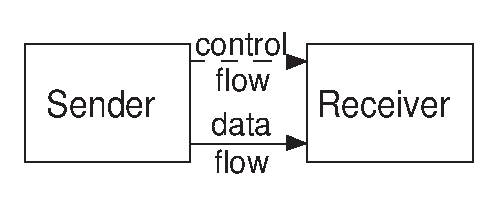
\includegraphics[width=.5\columnwidth]{pics/example}}
  \caption{Example figure}
  \label{fig:example}
\end{figure}

This template can be compiled with the \texttt{latex} command or the
\texttt{pdflatex} command. While \texttt{latex} creates an
intermediate file format (.dvi) that can be further processed into a
\texttt{.ps} or \texttt{.pdf} file, the \texttt{pdflatex} command
directly creates a \texttt{.pdf} file.

Note that with \texttt{latex} the \verb+\includegraphics+ accepts
only .eps files, while with \texttt{pdflatex} accepts \texttt{.pdf},
\texttt{.png}, or \texttt{.jpg}. Luckily, the file extension can be
omitted in order that \verb+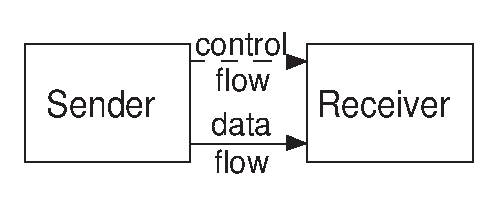
\includegraphics{pics/example}+ will
look for file with name \texttt{example.eps} in \texttt{latex} mode
and for a file with name \texttt{example.pdf}, \texttt{example.png},
or \texttt{example.jpg} in \texttt{pdflatex} mode. If you already
have an \texttt{.eps} file, you may create a respective
\texttt{.pdf} file with the commandline conversion tool
\texttt{epstopdf}.

\section{Citations and References}

Whenever you refer to previously published work, you should set a
reference to acknowledge the work you build upon. For example this
is a reference to two bachelor's theses~\cite{kraut:2003,
weirich:2005}. If you literally cite a part of someone else's work,
mark the respective sentence by quotes and italic letters and add
the page number, where is text can be found:

\dqit{An intelligent or {\em smart} transducer is the integration of
an analog or digital sensor or actuator element, a processing unit,
and a communication interface. In case of a sensor, the smart
transducer transforms the raw sensor signal to a standardized
digital representation, checks and calibrates the signal, and
transmits this digital signal to its users via a standardized
communication protocol.}\cite[p.\,175]{elmenreich:2005}

\section{Spellchecking}

Do not use your advisor as your spell checker. Instead, run an
electronic spell checker over your document before submitting the
document to your advisor.

\section{References with Bibtex}

Bibtex is an additional program to {\LaTeX} that creates a list of
your cited references in a chapter named {\em Bibliography}. In
order to use Bibtex, you must maintain a database of all references
in so-called \emph{bibfiles} (file extension \texttt{.bib}).

The \emph{bibfiles} contain entries of several types, the most
needed types are \texttt{book}, \texttt{inproceedings},
\texttt{article}, \texttt{techreport}, \texttt{mastersthesis}, and
\texttt{phdthesis}. In the following we list the templates for these
types, whereas each asterisk (*) should be replaced by the
respective data, if this is not available, the element should be
left out. The case of the element names does not matter to Bibtex,
however in the examples we have used UPPERCASE for the obligatory
fields and lowercase for the optional fields. To see some complete
examples, have a look into the file \texttt{bibfile.bib}. For more
information, read~\cite{patashnik:1988}.

\subsection{Some BibteX Examples}

\footnotesize
\begin{verbatim}
@BOOK{*,
  AUTHOR =       {*},
  editor =       {*},
  TITLE =        {*},
  PUBLISHER =    {*},
  YEAR =         {*},
  volume =       {*},
  number =       {*},
  series =       {*},
  address =      {*},
  edition =      {*},
  month =        {*},
  note =         {*}
}

@INPROCEEDINGS{*,
  AUTHOR =       {*},
  TITLE =        {*},
  BOOKTITLE =    {*},
  YEAR =         {*},
  editor =       {*},
  volume =       {*},
  number =       {*},
  series =       {*},
  pages =        {*},
  address =      {*},
  month =        {*},
  organization = {*},
  publisher =    {*},
  note =         {*}
}

@ARTICLE{*,
  AUTHOR =       {*},
  TITLE =        {*},
  JOURNAL =      {*},
  YEAR =         {*},
  volume =       {*},
  number =       {*},
  pages =        {*},
  month =        {*},
  note =         {*}
}

@TECHREPORT{*,
  AUTHOR =       {*},
  TITLE =        {*},
  INSTITUTION =  {*},
  YEAR =         {*},
  type =         {*},
  number =       {*},
  address =      {*},
  month =        {*},
  note =         {*}
}

@MASTERSTHESIS{*,
  AUTHOR =       {*},
  TITLE =        {*},
  SCHOOL =       {*},
  YEAR =         {*},
  type =         {*},
  address =      {*},
  month =        {*},
  note =         {*}
}

@PHDTHESIS{*,
  AUTHOR =       {*},
  TITLE =        {*},
  SCHOOL =       {*},
  YEAR =         {*},
  type =         {*},
  address =      {*},
  month =        {*},
  note =         {*},
  abstract =     {*},
  keywords =     {*},
  source =       {*},
} \end{verbatim}




%%
%% = eof =====================================================================
%%
+ & \verb+%%
%% Concepts
%%
%% This file should be edited by user
%%

\chapter{Concepts} \label{chapter:concepts}

Usually, this chapter is necessary in order to give an overview on
the \emph{terms} and \emph{concepts} that are required to understand
your work.

\section{Writing Style}

Usually you should not use the first person singular (\emph{I}) in
your text, write \emph{we} instead. As a general recommendation, use
the first person sparsely, sometimes it can be replaced by a phrase
like \emph{This work presents...}.

The indefinite article \textbf{a} is used as \textbf{an} before a
vowel sound - for example \textbf{an} apple, \textbf{an} hour,
\textbf{an} unusual thing, \textbf{an} FPGA (becourse the acronym is
pronouned Ef-Pee-Gee-A), \textbf{an} HIL. Before a consonant sound
represented by a vowel letter \textbf{a} is usual -- for example
\textbf{a} one, \textbf{a} unique thing, \textbf{a} historic
chance\footnote{According to Merriam Webster, both \textbf{a} and
\textbf{an} can be used in writing before unstressed or weakly
stressed syllables with initial h, thus you could also write
\textbf{an} historic chance.}.

\section{Acronyms}

Explain acronyms at their first occurrence in the text. In order to
achieve this consistently, we recommend to use the \texttt{acronym}
package.

A new acronym is then declared by writing
\verb+\newacro{acronym}{expanded name}+. Use the macro
\verb+\ac{acronym}+ as a placeholder for the acronym in the text.

See file \texttt{acronym.tex} for further examples and explanations.

\newacro{GPL}{Gnu Public License}

\section{Figures}

A Figure should always be referenced in the text, as it is the case
with Figure~\ref{fig:example}.

\begin{figure}[h]
 \centerline{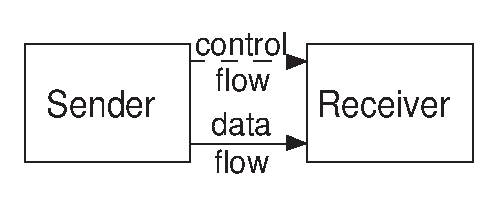
\includegraphics[width=.5\columnwidth]{pics/example}}
  \caption{Example figure}
  \label{fig:example}
\end{figure}

This template can be compiled with the \texttt{latex} command or the
\texttt{pdflatex} command. While \texttt{latex} creates an
intermediate file format (.dvi) that can be further processed into a
\texttt{.ps} or \texttt{.pdf} file, the \texttt{pdflatex} command
directly creates a \texttt{.pdf} file.

Note that with \texttt{latex} the \verb+\includegraphics+ accepts
only .eps files, while with \texttt{pdflatex} accepts \texttt{.pdf},
\texttt{.png}, or \texttt{.jpg}. Luckily, the file extension can be
omitted in order that \verb+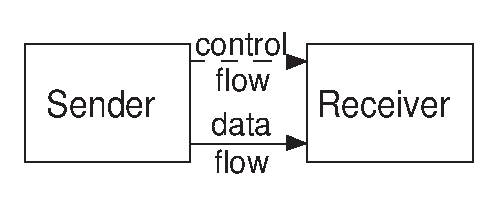
\includegraphics{pics/example}+ will
look for file with name \texttt{example.eps} in \texttt{latex} mode
and for a file with name \texttt{example.pdf}, \texttt{example.png},
or \texttt{example.jpg} in \texttt{pdflatex} mode. If you already
have an \texttt{.eps} file, you may create a respective
\texttt{.pdf} file with the commandline conversion tool
\texttt{epstopdf}.

\section{Citations and References}

Whenever you refer to previously published work, you should set a
reference to acknowledge the work you build upon. For example this
is a reference to two bachelor's theses~\cite{kraut:2003,
weirich:2005}. If you literally cite a part of someone else's work,
mark the respective sentence by quotes and italic letters and add
the page number, where is text can be found:

\dqit{An intelligent or {\em smart} transducer is the integration of
an analog or digital sensor or actuator element, a processing unit,
and a communication interface. In case of a sensor, the smart
transducer transforms the raw sensor signal to a standardized
digital representation, checks and calibrates the signal, and
transmits this digital signal to its users via a standardized
communication protocol.}\cite[p.\,175]{elmenreich:2005}

\section{Spellchecking}

Do not use your advisor as your spell checker. Instead, run an
electronic spell checker over your document before submitting the
document to your advisor.

\section{References with Bibtex}

Bibtex is an additional program to {\LaTeX} that creates a list of
your cited references in a chapter named {\em Bibliography}. In
order to use Bibtex, you must maintain a database of all references
in so-called \emph{bibfiles} (file extension \texttt{.bib}).

The \emph{bibfiles} contain entries of several types, the most
needed types are \texttt{book}, \texttt{inproceedings},
\texttt{article}, \texttt{techreport}, \texttt{mastersthesis}, and
\texttt{phdthesis}. In the following we list the templates for these
types, whereas each asterisk (*) should be replaced by the
respective data, if this is not available, the element should be
left out. The case of the element names does not matter to Bibtex,
however in the examples we have used UPPERCASE for the obligatory
fields and lowercase for the optional fields. To see some complete
examples, have a look into the file \texttt{bibfile.bib}. For more
information, read~\cite{patashnik:1988}.

\subsection{Some BibteX Examples}

\footnotesize
\begin{verbatim}
@BOOK{*,
  AUTHOR =       {*},
  editor =       {*},
  TITLE =        {*},
  PUBLISHER =    {*},
  YEAR =         {*},
  volume =       {*},
  number =       {*},
  series =       {*},
  address =      {*},
  edition =      {*},
  month =        {*},
  note =         {*}
}

@INPROCEEDINGS{*,
  AUTHOR =       {*},
  TITLE =        {*},
  BOOKTITLE =    {*},
  YEAR =         {*},
  editor =       {*},
  volume =       {*},
  number =       {*},
  series =       {*},
  pages =        {*},
  address =      {*},
  month =        {*},
  organization = {*},
  publisher =    {*},
  note =         {*}
}

@ARTICLE{*,
  AUTHOR =       {*},
  TITLE =        {*},
  JOURNAL =      {*},
  YEAR =         {*},
  volume =       {*},
  number =       {*},
  pages =        {*},
  month =        {*},
  note =         {*}
}

@TECHREPORT{*,
  AUTHOR =       {*},
  TITLE =        {*},
  INSTITUTION =  {*},
  YEAR =         {*},
  type =         {*},
  number =       {*},
  address =      {*},
  month =        {*},
  note =         {*}
}

@MASTERSTHESIS{*,
  AUTHOR =       {*},
  TITLE =        {*},
  SCHOOL =       {*},
  YEAR =         {*},
  type =         {*},
  address =      {*},
  month =        {*},
  note =         {*}
}

@PHDTHESIS{*,
  AUTHOR =       {*},
  TITLE =        {*},
  SCHOOL =       {*},
  YEAR =         {*},
  type =         {*},
  address =      {*},
  month =        {*},
  note =         {*},
  abstract =     {*},
  keywords =     {*},
  source =       {*},
} \end{verbatim}




%%
%% = eof =====================================================================
%%
+ \\
  \verb+\cleardoublepage+ & \verb+\cleardoublepage+ \\
  \verb+%%
%% Related Work
%%
%% This file should be edited by user
%%

\chapter{Related Work} \label{chapter:relatedwork}

This chapter should give an overview over existing work that is
related to your work. Instead of \dq{Related Work}, this chapter can
also be named specifically to the topic of the thesis.

For example in Bernhard Weirich's Bachelor's thesis, there are two
chapters on related work named \dq{Time-Driven Algorithms} and
\dq{Event-Driven Algorithms}~\cite{weirich:2005}.

Each related approach should be described by a section of about
100-500 words.

\section{Types of Bachelor's Theses}

If you write a plain report on some implementation, you might have
no chapter on related works.

%%
%% = eof =====================================================================
%%
+ & \verb+%%%
%% Related Work
%%
%% This file should be edited by user
%%

\chapter{Related Work} \label{chapter:relatedwork}

This chapter should give an overview over existing work that is
related to your work. Instead of \dq{Related Work}, this chapter can
also be named specifically to the topic of the thesis.

For example in Bernhard Weirich's Bachelor's thesis, there are two
chapters on related work named \dq{Time-Driven Algorithms} and
\dq{Event-Driven Algorithms}~\cite{weirich:2005}.

Each related approach should be described by a section of about
100-500 words.

\section{Types of Bachelor's Theses}

If you write a plain report on some implementation, you might have
no chapter on related works.

%%
%% = eof =====================================================================
%%
+ \\
  \verb+\cleardoublepage+ & \verb+%\cleardoublepage+ \\
  \verb+%%
%% Design Approach
%%
%% This file should be edited by user
%%

\chapter{Design Approach} \label{chapter:designapproach}

If you have derived some new concepts on your own, this is the place
to present them. You can use generic names for this chapter like
\dq{Design Approach} or \dq{System Architecture} or chose name
accordingly to its contents (for example \dq{Automatic Text
Generator Algorithm}).

\section{Types of Bachelor's Theses}

If you write a Bachelor's thesis in form of a survey, you might have
several chapters on existing work from others, but no chapter as
described here.


%%
%% = eof =====================================================================
%%
+ & \verb+%%
%% Design Approach
%%
%% This file should be edited by user
%%

\chapter{Design Approach} \label{chapter:designapproach}

If you have derived some new concepts on your own, this is the place
to present them. You can use generic names for this chapter like
\dq{Design Approach} or \dq{System Architecture} or chose name
accordingly to its contents (for example \dq{Automatic Text
Generator Algorithm}).

\section{Types of Bachelor's Theses}

If you write a Bachelor's thesis in form of a survey, you might have
several chapters on existing work from others, but no chapter as
described here.


%%
%% = eof =====================================================================
%%
+ \\
  \verb+\cleardoublepage+ & \verb+\cleardoublepage+ \\
  \hline
\end{tabular}
\end{center}
  \caption{Removing the Chapter \texttt{Related Work}}\label{table:removing}
\end{table}

\subsection{Adding Chapters} \label{section:addingchapters}

Open the file \texttt{thesis.tex} and add an
\verb+\include{+\emph{filename}\verb+}+ command (followed by a
\verb+\cleardoublepage+) at the respective line. Then create a new
file \emph{filename}\verb+.tex+ in the same directory and write the
chapter's contents into it.

\subsection{Adding References} \label{section:addingreferences}

Whenever you \verb+\cite+ something, there must be a respective
entry in any of the included .bib files. To add such an entry, open
the respective bibfile (\eg \texttt{bibfile.bib}) with a text editor
and add the entry according to the bibfile syntax. The reference
will be added after running latex/bibtex/latex on your project.

\subsection{Removing References} \label{section:removingreferences}

Remove all \verb+\cite+ commands to this reference in the text and
the citation will not be listed in the bibliography after running
latex/bibtex/latex on your project. There is no need to remove the
reference from the .bib file.

\subsection{Changing the .bib Files to be used}

In the file \texttt{thesis.tex} there is a line with a
\verb+\bibliography+ command, that lists all used .bib files without
file extensions separated by commas.

\subsection{Troubleshooting}

If you make something wrong, you should get an error at compile
time, except for citation problems, like:

\begin{description}
\item[Adding or removing references does not work:]~~Perhaps there is
a spelling error in some .bib file, this causes the program
\texttt{bibtex} to abort execution leaving the old bibliography
unchanged.

\item[Changing a reference does not work:]~~Some systems only perform
a new bibtex run if there are missing references, delete the
\texttt{.aux} file in order to overcome this problem.

\item[References show a question mark:]~~Bibtex could not find a
matching entry in the bibfile for this reference, check the label
name.

\end{description}



%%
%% = eof =====================================================================
%%
